\chapter{Introduction}
\label{cap:intro}

Traditional computer networks have been successful in their most basic goal: making packets originated from a source location reach a destination \cite{Shenker95fundamentaldesign}. However, with the exponential growth in Internet users, emerging use cases and applications have become a challenge for network carriers and administrators. These professionals should be able to handle and to master more and more complex scenarios and configurations \cite{Feldmann:2007:ICD:1273445.1273453}. Furthermore, network equipments are strictly closed or only offer a small set of options for users who want to add their own functionalities and applications. Consequently, innovation in computer networks is compromised, compelling companies to wait for new features on software updates or, worse, to buy a new network box. 

In order to address these issues, inspired by older technologies that have followed similar concepts and evolved \cite{Feamster:2014:RSI:2602204.2602219}, a new network model was designed. The Software Defined Networking (SDN) \cite{DBLP:journals/corr/KreutzRVRAU14}, is a network architecture in which the control plane of network switches is decoupled from the forwarding plane, as illustrated by Figure 1. The control plane is responsible for the management of one or more elements from the forwarding plane. The applications running on top of the control plane can program the data plane to execute determined actions according to the packet type received by an equipment or some network event. As a result of this flexibility to control the forwarding plane, network equipments may receive new functions and do not need to be replaced when the need for a new functionality arises. Moreover, the network resources can be fully exploited by some smart resource allocation, like network virtualization \cite{FLOWVISOR} \cite{Al-Shabibi:2014:OMY:2620728.2620741}, leveraging the network to its full potential.

\begin{figure}[h!]
\centering
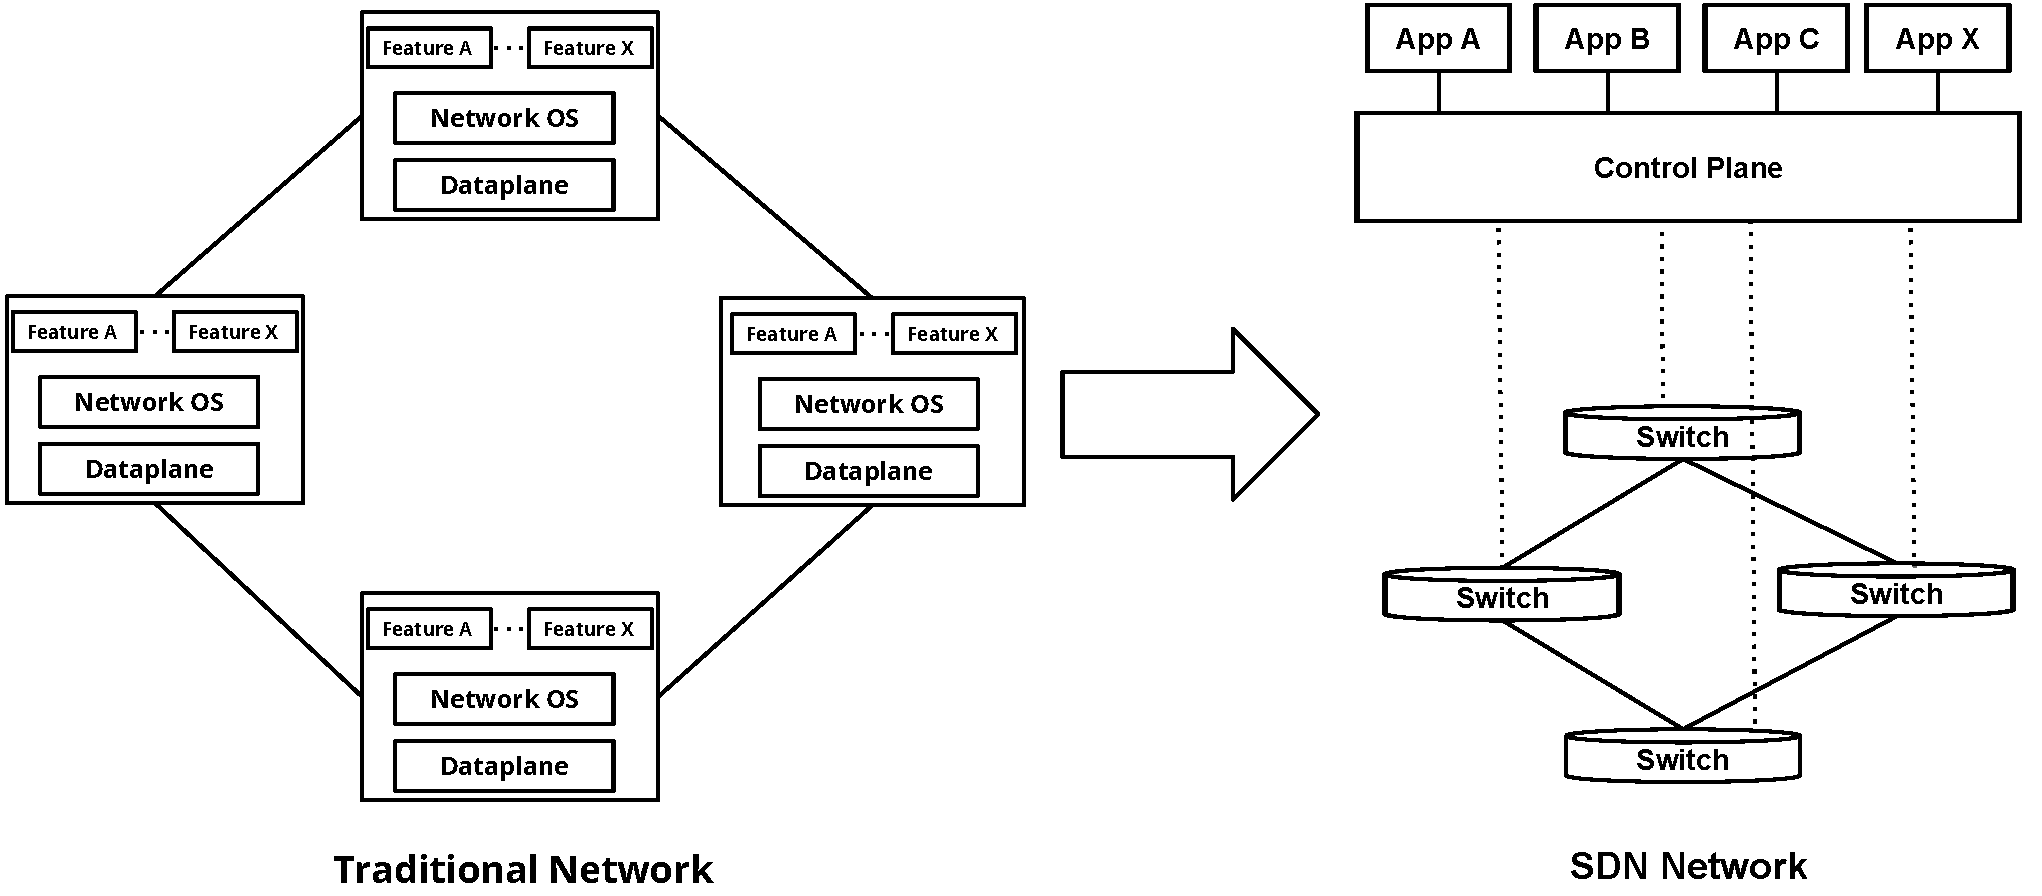
\includegraphics[width=\textwidth,keepaspectratio]{cap1/TraditionalvsSDN.pdf}
\caption{Traditional and SDN models}
\label{fig:traditional_vs_sdn}
\end{figure}
    
In Software Defined Networks, communication between the control and data plane relies in some sort of protocol or Application Command Interface (API), also known as southbound API. The first and the most common standard southbound interface for SDN is the OpenFlow protocol \cite{McKeown:2008:OEI:1355734.1355746} \cite{2012onf_sdn}. The OpenFlow specification describes the interaction between an OpenFlow compliant switch and an OpenFlow controller. Basically, through OpenFlow messages a controller can program the switches forwarding logic based on the type of packets transiting the network.     

\section{Motivation}
\label{sec:sec01}

Among the reasons for the fast evolution of the OpenFlow protocol is the experimental work led by researchers from Stanford, where the protocol was born. New features and capabilities were validated on a software switch implementation, allowing researchers to create and to try new control plane applications. Soon, advances and emerging use cases took the industry attention for SDN and OpenFlow. This culminated in the creation of the Open Network Foundation (ONF), an organization composed by big network players and vendors, as by emerging startups. This organization became responsible for new OpenFlow versions since the version 1.2 and started working on new and enhanced features, resulting in the version 1.3 less than one year after 1.2. 

On the other hand, OpenFlow controllers and switches did not follow the protocol advancements, notwithstanding the fast evolution, resulting in lack of alternatives to experiment new capabilities and anticipation of new applications that could benefit from new features.

With this scenario in mind we found the emerging need to upgrade these tools, allowing fast experimentation and validation. By keeping up the pace with OpenFlow new versions, we expect to contribute to the future of the protocol, driving companies and researchers to develop applications in the state of the art and  enabling future OpenFlow version to be build and tested upon our work.  

\section{Objectives}
\label{sec:sec02}

The objective of this work is the development of a programmable OpenFlow 1.3 software switch to enable fast, real and flexible experimentation for SDN research and education on OpenFlow networks. To achieve this, the software switch must meet the following requirements:  

\begin{enumerate}

\item  \textbf{OpenFlow protocol feature completeness.} All required and optional features shall be implemented, allowing a full OpenFlow experience, without limitations for SDN researchers and developers.   

\item  \textbf{Code simple, easy to prototype and extend.} The code must be simple enough to be modified by anyone with a basic level of programming and understanding of OpenFlow. For this reason, easy insertion of features should be favored in lieu of performance. This requisite meets research needs that goes beyond the OpenFlow specification (e.g: the addition of new messages, new algorithms for group processing, changes to the pipeline, etc). Also, it encourages and helps users to search and to fix bugs quickly, preventing work interruption while waiting for an official patch to correct the switch.       

\item  \textbf{Straight forward integration with experimentation environments and emulation tools.} The switch must integrate with both real and emulated environments, ensuring seamless communication with other switches and controllers, without great modifications. Minor changes are acceptable due to specific platforms requirements: for instance, different processor architectures.

\begin{savenotes}
    \begin{table}[h!]
    \centering
    \caption{Minimum bandwidth requirements for common internet applications}
    \label{tab:appband}
    \begin{tabular}{|l|l|l|}
    \hline
    \textbf{Application}          & \textbf{Bandwidth (Mbps)}                         \\ \hline
    Web Browsing                      & 0.038                                        \\ \hline
    Email                             & 0.01                                          \\ \hline
    Telnet                            & < 0.001                                          \\ \hline
    Audio Broadcasting                & 0.08 to 0.375\footnote{Spotify - https://support.spotify.com/us/learn-more/faq/\#!/article/What-bitrate-does-Spotify-use-for-streaming}                                          \\ \hline
    Video Broadcasting                & 0.5 to 60 \footnote{Netflix - https://help.netflix.com/en/node/306}                                          \\ \hline
    
    \end{tabular}
    \end{table}
\end{savenotes}

\item \textbf{Maximum throughput equal or higher than 100 Mbps.} High performance is not one of the project goals. However, there are features that play with the switch packet rate. Therefore, for a significant user experience, the switch must be able to support rates of at least 100 Mbps. This value was estimated based by the minimum bandwidth required by common Internet applications. Table \ref{tab:appband} is a mix from values obtained by \cite{Chen:2004:QRN:1234242.1234243} and some popular Internet services. Considering the applications and the bandwidth usage, we found that 100 Mbps is a value to perform a reasonable number of different experiments.          

\end{enumerate}




\section{Text Structure}
\label{sec:sec03}

In this Introduction we explained the motivational aspects that justify this work. Also, we give a clear explanation for the objectives of this project. 

In Chapter~\ref{cap:cap02} we present a Literature Review. Related OpenFlow software switches' current functionalities are discussed from the point of view of our implementation requisites. Furthermore, we introduce other tools which are important parts of the OpenFlow ecosystem. 

In Chapter~\ref{cap:cap03} we take a look at the architecture of the software switch which is compliant with OpenFlow 1.3. We explain the modules relationship and roles within the OpenFlow pipeline.

In Chapter~\ref{cap:cap04} we highlight implementation details of OpenFlow 1.3 features in our architecture.  

In Chapter~\ref{cap:cap05} we evaluate the software switch in terms of common OpenFlow benchmarks and compare with related work.

Finally, in Chapter~\ref{cap:conclusion} we give our conclusion remarks. This chapter highlights results, presents known use cases and discusses possible improvements in future works. 

